\documentclass{beamer}
\usepackage{amsmath}
\usepackage{amssymb}
\usepackage{booktabs}
\usepackage{rotating}
\usepackage{multirow}
\usepackage{colortbl,color}
\usepackage{graphics}

\usepackage{colortbl,color}
\usetheme{material}
\useLightTheme
\usePrimaryRed
\useAccentGreen

\renewcommand{\theenumii}{\alph{\enumii}}
\defbeamertemplate{itemize subitem}{dash}{--}
\defbeamertemplate{itemize subsubitem}{dash}{--}
\setbeamertemplate{itemize item}[circle]
\setbeamertemplate{itemize subitem}[dash]
\setbeamertemplate{itemize subsubitem}[dash]
\setbeamertemplate{enumerate item}{\arabic{enumi}.}
\setbeamertemplate{enumerate subitem}{(\alph{enumii})}
\usefoottemplate{}

\setbeamertemplate{headline}{}
\usenavigationsymbolstemplate{}

\newcommand{\UNCOVER}[3]{\only<#2>{\color{white}{#1}}\only<#3>{#1}}
\newcommand{\UNCOVERR}[4]{\only<#2>{\color{white}{#1}}\only<#3>{\color{red}{#1}}\only<#4>{#1}}
\newcommand{\showOn}[3]{\only<#2>{\color<#2>{black} #1}\only<#3>{\color<#3>{white} #1}}
\newcommand{\SD}[1]{{\tiny $\left(#1\right)$}}
\newcommand{\SDm}[1]{{\tiny \left(#1\right)}}
\newcommand{\Prob}[1]{\mbox{Pr}\left\{#1\right\}}
\newcommand{\CProb}[2]{\mbox{Pr}\left\{#1\left|#2\right.\right\}}

\usepackage{array}
\newcolumntype{P}[1]{>{\centering\arraybackslash}p{#1}}


\newcommand{\indicator}[1]{\mathrm{1}\left\{{#1}\right\}}

\begin{document}

    \date{Fall 2020}
    \title{Honesty on the Margin(s)}
    \author{Alistair Wilson\and  (with Johnathan Lafky, Simon Halliday)}
    \maketitle

\begin{frame}{Introduction}
    \begin{itemize}
        \item Well-published experimental literature identifying a preference for
        honesty
            \begin{itemize}
                \item Initial paradigms: Gneezy (AER, 2006), Fischbacher \& Folmi-Heusi
                (JEEA 2013)
                \item Modeling: Gneezy et al (AER, 2018); Dufwenberg$^{2}$(JET 2018); Abeler
                et al. (ECMA, 2019)
            \end{itemize}
        \item If preferences for honesty are a robust feature of decision making, this opens up the possibility for a lot of very interesting economic comparative statics, alternative policies, mechanism-design possibilities, etc.\pause
        \item But what happens in richer environments
            \begin{itemize}
                \item We look at two types of endogeneity: \emph{Self-Selection} and \emph{Competition}
                \item Examine the effects within the standard experimental paradigm
            \end{itemize}
    \end{itemize}
\end{frame}

\begin{frame}{Introduction}
    \begin{itemize}
        \item Lying preferences have mostly been identified through decision problems
            \begin{itemize}
                \item Experimental literature with repetition in strategic sender-receiver games finds greater rates of dishonesty (though still substantial honesty)
                \item Even for repeated sender-receiver games where honesty is possible in equilibrium, there is not substantial evidence for it (Vespa \& Wilson), where other features of the strategic setting dominate
            \end{itemize}
        \item Wanted to better understand the domains for which lying averse preferences
        are useful\pause 
            \begin{itemize}
                \item Which economic/equilibrium forces break the standard result? Which
                don't?
                \item Can the literature models help us understand why...
            \end{itemize}
    \end{itemize}
\end{frame}


\begin{frame}{Our Experiment and Result Spoiler}
    \begin{itemize}
        \item Our experiment modifies the Fischbacher \& F\"ollmi-Heusi (JEEA 2013) die-rolling task which we repeat many times to allow convergence to steady state (the limit of the title)
            \begin{itemize}
                \item \textbf{Competition}: Match participants to either a robot player or another participant
                \item \textbf{Selection:} Introduce an outside-option task with a fixed payoff
            \end{itemize}
        \item Two margins: \emph{Intensive} (honesty) and\emph{ Extensive} (task choice)
    \end{itemize}
\end{frame}


\begin{frame}{Economic frame}
    \begin{itemize}
        \item Consider a profession where lying/exaggerating can increase the individual's
        payoff
            \begin{itemize}
                \item Salespeople
                \item Politicians
            \end{itemize}
        \item Natural endogeneities:
            \begin{itemize}
                \item Population: those in the profession are self selected
                \item Returns: payoffs depend on others' behavior
            \end{itemize}
    \end{itemize}
\end{frame}

\begin{frame}
    \begin{itemize}
        \item Motivating questions:
            \begin{enumerate}
                \item What happens (within the standard experimental construct) as we allow each force to equilibriate
                \item Can the preference model identified by the decision problems help us understand the economic forces that lead us to qualitatively distinct results
            \end{enumerate}
    \end{itemize}
\end{frame}

\begin{frame}{Experimental Task}
    \begin{itemize}
        \item In each round subjects choose between two tasks:
            \begin{itemize}
                \item \textbf{Fixed}
                \item \textbf{Competitive}
            \end{itemize}
        \item After choosing their task, they privately roll a 10-sided die and
        report the result 0\textendash 9
            \begin{itemize}
                \item \textbf{Competitive}: win \$15 prize if their roll is higher than a matched roll, \$5 otherwise
                \item \textbf{Fixed}: Win the \$15 prize if their roll matches the parity (odd/even) of a computer roll
            \end{itemize}
        \item Repeat the task 30 times
            \begin{itemize}
                \item Feedback only given within the chosen task
            \end{itemize}
    \end{itemize}
\end{frame}

\begin{frame}{Experimental Design}

Three-by-two between-subject design:
    \begin{itemize}
        \item \textbf{Outside option}
            \begin{itemize}
                \item No Selection (No fixed task)
                \item Low ($u_{0}=0.25$)
                \item High ($u_{0}=0.45$)
            \end{itemize}
        \item \textbf{Payoffs:}
            \begin{itemize}
                \item \emph{Exogenous} \textrm{$\pi(x)$}: matched to honest computer roll
                \item \emph{Endogenous} \textrm{$\pi^{\star}(x)$}: matched to random competitive-task roll
            \end{itemize}
    \end{itemize}
\end{frame}

\begin{frame}{Round Timing}
    \begin{enumerate}
        \item Subject chooses a task: \emph{Fixed} or \emph{Competitive}
        \item Subjects roll 10-sided dies and report the result (0\textendash 9)
        \item Outcomes are realized:
    \end{enumerate}
\end{frame}

\begin{frame}{Fixed Task in Low/High treatments}
    \begin{itemize}
        \item Subject rolls their die; report result $X$
        \item After report, computer draws a ball from an urn with 100 balls
            \begin{itemize}
                \item $n$ balls labeled \emph{Odd}
                \item $n$ balls labeled \emph{Even}
                \item $5$ balls labeled \emph{Any}
                \item $95-2n$ balls labeled \emph{Neither}
            \end{itemize}
        \item Round earnings of \$15 if ball matches their die roll, \$5 otherwise
            \begin{itemize}
                \item Expected probability of $p=\frac{n+5}{100}$ to win \$15 prize for
                all die rolls
                \item High outside option, $n=40$ $\Rightarrow u_{0}=0.45$
                \item Low outside option, $n=20$ $\Rightarrow u_{0}=0.25$
            \end{itemize}
    \end{itemize}
\end{frame}

\begin{frame}{Competitive Task}
    \begin{itemize}
        \item Matched to another roll ($X$), where highest roll gets \$15, lowest
        \$5, ties broken by coin flip
        \item Ex-ante payoff from report $x$ given by 
        \[
        \pi(x)=\tfrac{1}{2}\Pr\{x=X\}+\Pr\{x>X\}\cdot
        \]
    \end{itemize}
    \begin{description}
        \item [{Exogenous:}] $X$ a D10 Roll made by the computer, linear payoff
        $\pi(x)=\tfrac{1}{20}+\tfrac{1}{10}x$
        \item [{Endogenous:}] $X^{\star}$ a D10 report from another participant
        that also opted into competitive task
    \end{description}
\end{frame}

\begin{frame}{Experiment Details}
    \begin{itemize}
        \item University of Pittsburgh undergraduate subjects
        \item Conducted at the PEEL Lab
        \item Paid for two random decisions over 30 rounds (no show-up)
            \begin{itemize}
                \item Payoffs are either \$10, \$20 or \$30
            \end{itemize}
        \item 288 Subjects:
            \begin{itemize}
                \item $72\times3$ Subjects for each Endog-$\pi^{\star}$ treatment
                \item $24\times3$ Subjects for each Exog-$\pi$ treatment
            \end{itemize}
    \end{itemize}
\end{frame}

% \begin{frame}{Design model (tractable)}
%     \begin{itemize}
%         \item Going into this project we had a simple (and importantly, tractable)
%         model that guided our hypotheses:
%         \[
%         \begin{array}{ccccc}
%         \text{Utility} & = & \text{Payoff} & - & \text{Lying Cost}\\
%         U_{i}(\omega,x;\theta_{i}) & = & \pi(x) & - & \theta_{i}\cdot\boldsymbol{1}_{\omega\not=x}\cdot c
%         \end{array}
%         \]
%             \begin{itemize}
%                 \item where $\theta_{i}$ is an individual's lying cost, drawn from a distribution
%             $F(\theta)$ with support $[0,\kappa]$\pause 
%             \end{itemize}
%         \item Comparative statics:
%                 \begin{itemize}
%                     \item No effect from the outside option (full entry) with exogenous payoffs
%                     \item With endogenous payoffs: honesty levels are either unaffected by the
%                     outside option, or fully dishonest
%                     \item Honest behavior less stable the greater is $u_{0}$
%             \end{itemize}
%     \end{itemize}
% \end{frame}

\begin{frame}{Lying Models: Lying Cost+Reputation}
    \begin{itemize}
        \item Abeler et al. meta study calibrated preference model:
        \[
        \begin{array}{ccccccc}
        \text{Utility} & = & \text{Payoff} & - & \text{Lying Cost} & - & \text{Reputation Cost}\\
        U_{i}(\omega,x;\theta_{i}) & = & \pi(x) & - & \boldsymbol{1}_{\omega\not=x}\cdot c & - & \theta_{i}\cdot\Lambda^{\star}(x)
        \end{array}
        \]
        \begin{itemize}
            \item $\Lambda^{\star}(x)$ is the proportion of liars making report $x$
            \item $\theta_{i}$ is instead the individual's cost parameter for reputation
            loss
            \item $c>0$ is a fixed lying cost
            \item Population is given by $\theta_{i}\sim U[0,\kappa]$
        \end{itemize}
    \end{itemize}
\end{frame}

\begin{frame}{Exogenous/Standard set-up}
    \begin{itemize}
        \item Taking the meta-study's calibrated parameters for the LC+Reputation model ($c=\tfrac{27}{50}$ and $\kappa=2$) without any endogeneities compares well with the prediction
    \end{itemize}
    \begin{center}
    	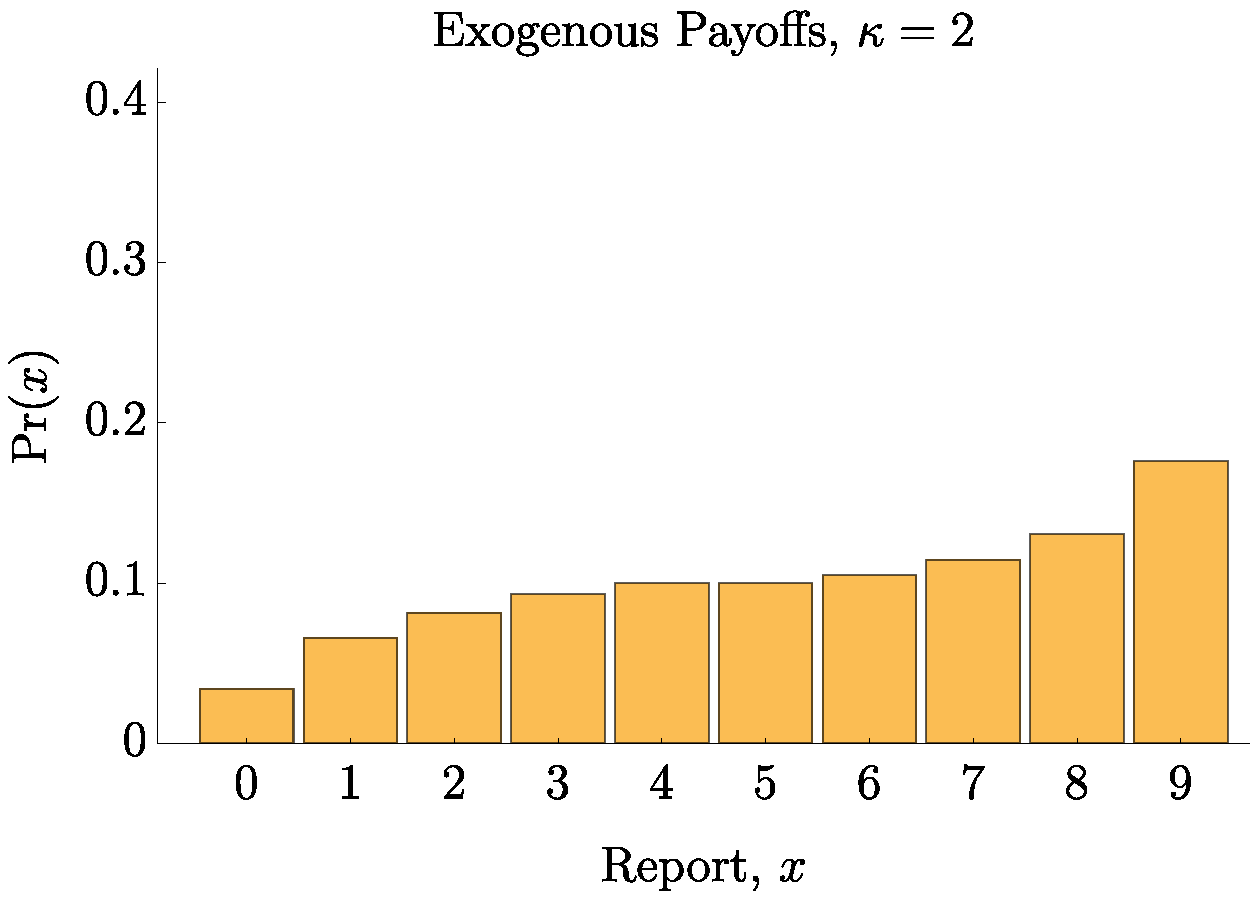
\includegraphics[width=0.49\textwidth]{./ih/pred_hist_ex_2.pdf}
    	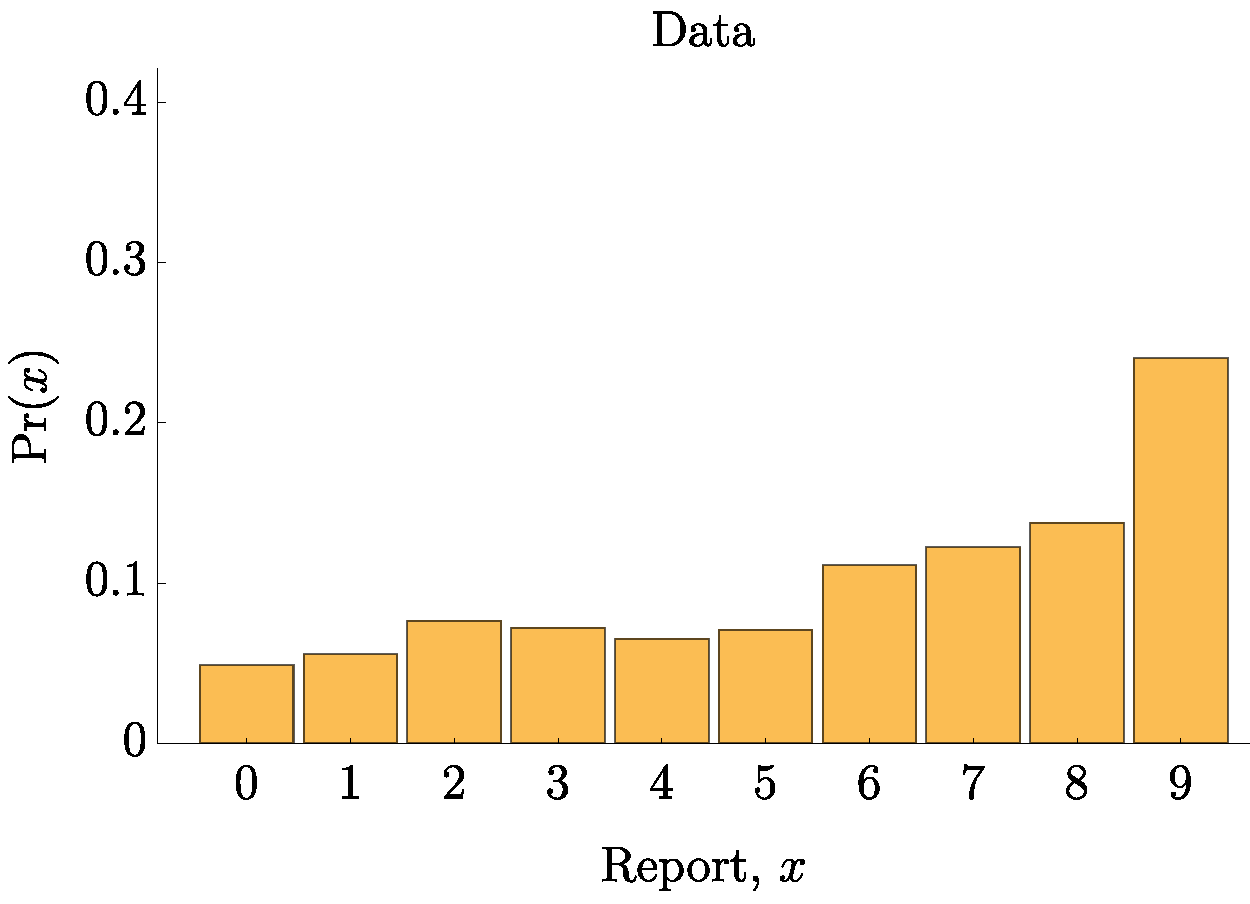
\includegraphics[width=0.49\textwidth]{./ih/emp_hist_ex_nolabel.pdf}
    \end{center}
\end{frame}

\begin{frame}{Questions}
    \begin{eqnarray*}
    U_{i}(\omega,x;\theta) & = & \pi(x)-\boldsymbol{1}_{\omega\not=x}\cdot c-\theta_{i}\cdot\Lambda^{\star}(x)\\
     & \text{} & \text{where},\theta_{i}\sim U[0,\kappa]
    \end{eqnarray*}

    \begin{itemize}
        \item What does the model predict as we endogenize:
            \begin{itemize}
                \item \textbf{Population:} the $\theta$-types that participate: $\Rightarrow\kappa\rightarrow\kappa^{\star}$
                \item \textbf{Payoffs:} the return to each report: $\Rightarrow\pi(x)\rightarrow\pi^{\star}(x)$
                \item \textbf{Both}: $\Rightarrow\left(\kappa,\pi\left(x\right)\right)\rightarrow\left(\kappa^{\star},\pi^{\star}\left(x\right)\right)$
            \end{itemize}
    \end{itemize}
\end{frame}

\begin{frame}{Selection}
    \begin{eqnarray*}
    U_{i}(\omega,x;\theta) & = & \pi(x)-\boldsymbol{1}_{\omega\not=x}\cdot c-\theta_{i}\cdot\Lambda^{\star}(x)\\
     & \text{} & \text{where},\theta_{i}\sim U[0,\kappa]
    \end{eqnarray*}
    
    \begin{itemize}
        \item Fixed setting: given preferences can calculate equilibrium:
            \begin{itemize}
                \item $\xi_{\theta}(\omega)$: action by reputation type $\theta$
                \item $\Lambda^{\star}(x):$ fraction of liars at each report
            \end{itemize}
        \item Provide an outside option $u_{0}$
        \item Ex ante expected payoff is:
        \begin{eqnarray*}
            \mathbb{E}U(\theta) & = & \mathbb{E}U_{i}\left(\omega,\xi_{\theta}\left(\omega\right)\right)\\
         & = & \mathbb{E}\text{Payoff}-c\cdot\text{LyingRate}(\theta)-\theta_{i}\cdot\text{\ensuremath{\mathbb{E}}RepCost}(\theta)
        \end{eqnarray*}
    \end{itemize}
\end{frame}

\begin{frame}{Theory: Expected Payoff by Reputation Cost}
    \begin{center}
        \includegraphics<1>[width=0.9\textwidth]{./ih/ExpectUtilityRep0.pdf}
        \includegraphics<2>[width=0.9\textwidth]{./ih/ExpectUtilityRep1.pdf}
        \includegraphics<3>[width=0.9\textwidth]{./ih/ExpectUtilityRep2.pdf}
    \end{center}
\end{frame}

\begin{frame}{Selection effects}
    \begin{eqnarray*}
    U_{i}(\omega,x;\theta) & = & \pi(x)-\boldsymbol{1}_{\omega\not=x}\cdot c-\theta_{i}\cdot\Lambda^{\star}(x)\\
     & \text{} & \text{where},\theta_{i}\sim U[0,\kappa]
    \end{eqnarray*}

    \begin{itemize}
    \item Self-selection in the model is equivalent to solving for an equilibrium
    $(\xi^{\star},\Lambda^{\star},\kappa^{\star})$
        \begin{itemize}
            \item where $u_{0}=\mathbb{E}U(\kappa^{\star})$
        \end{itemize}
    \end{itemize}
\end{frame}

\begin{frame}{Selection effects}
    \begin{eqnarray*}
        U_{i}(\omega,x;\theta) & = & \pi(x)-\boldsymbol{1}_{\omega\not=x}\cdot c-\theta_{i}\cdot\Lambda^{\star}(x)\\
     & \text{} & \text{where},\theta_{i}\sim U[0,\kappa]
    \end{eqnarray*}
    \begin{itemize}
        \item Self-selection in the model is equivalent to solving for an equilibrium
        $(\xi^{\star},\Lambda^{\star},\kappa^{\star})$
            \begin{itemize}
                \item $u_{0}=H$$,\rightarrow$ $\kappa^{\star}\approx\text{\ensuremath{\min}\{}1,\kappa\}$
                \item $u_{0}=L$$,\rightarrow$ $\kappa^{\star}\approx\text{\ensuremath{\min}\{}5,\kappa\}$
            \end{itemize}
    \end{itemize}
\end{frame}

\begin{frame}{Selection Effects}
    \begin{center}
        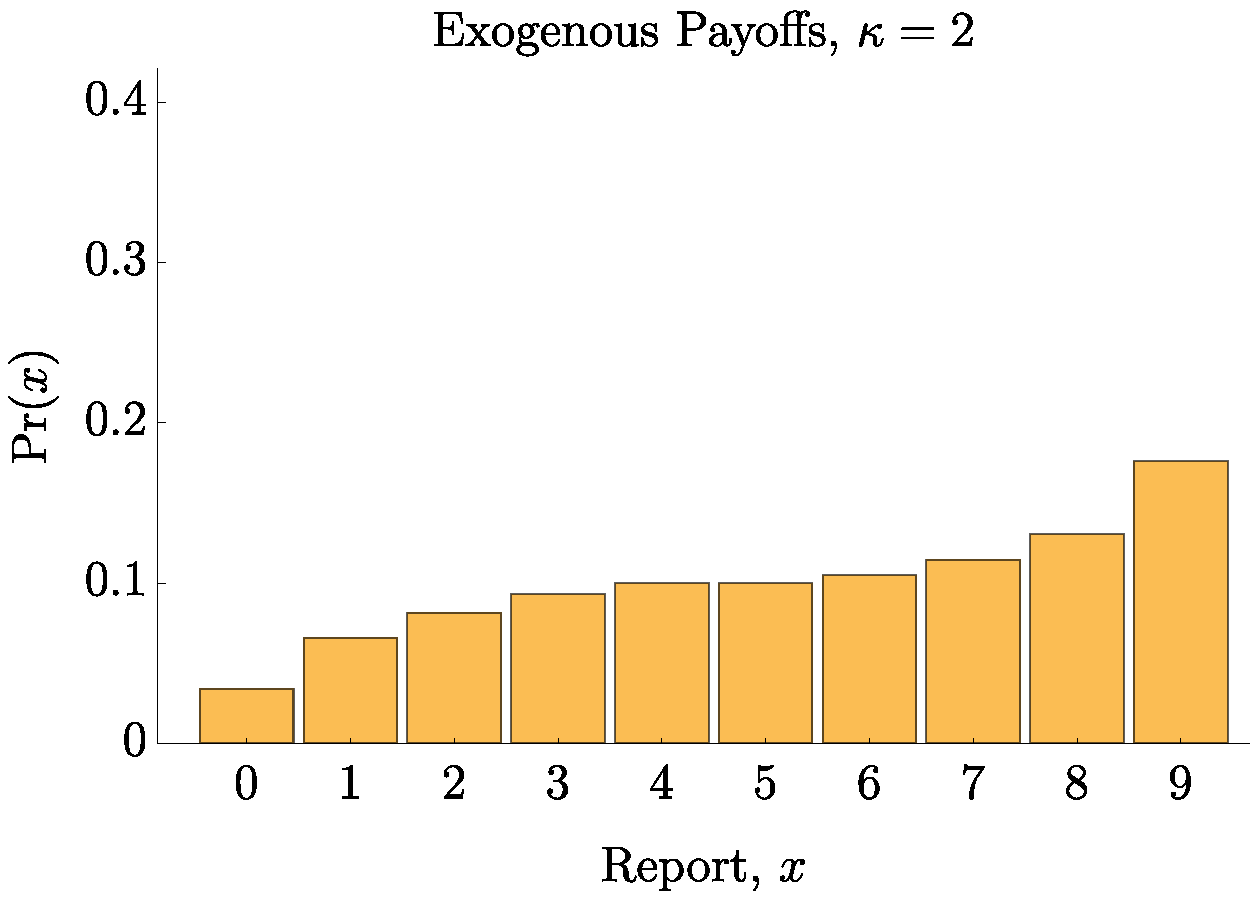
\includegraphics[width=0.4\textwidth]{./ih/pred_hist_ex_2.pdf}
        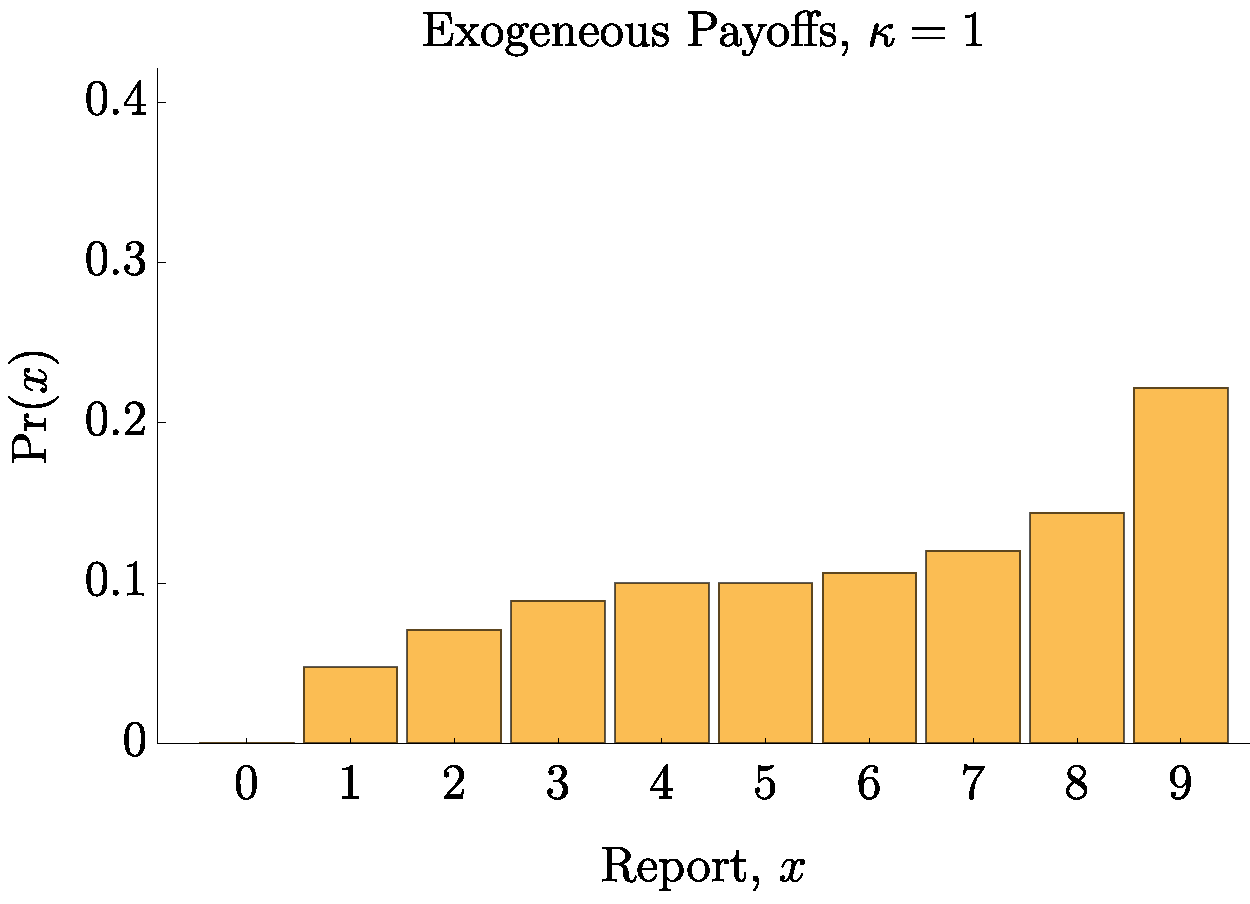
\includegraphics[width=0.4\textwidth]{./ih/pred_hist_ex_1.pdf}
    \end{center}
\end{frame}

\begin{frame}{Competition effects}
    \begin{eqnarray*}
    U_{i}(\omega,x;\theta) & = & \pi^{\star}(x)-\boldsymbol{1}_{\omega\not=x}\cdot c-\theta_{i}\cdot\Lambda^{\star}(x)\\
     & \text{} & \text{where},\theta_{i}\sim U[0,\kappa]
    \end{eqnarray*}

    \begin{itemize}
        \item Endogenizing payoffs through competition shifts payoffs
        \[
        \Pr(x_{i}=\omega_{j})+\Pr(x>\omega_{j})\rightarrow\Pr\left(x=\xi^{\star}(\omega_{j})\right)+\left(x=\xi^{\star}(\omega_{j})\right)
        \]
        \item Competitive payoffs requires us to solve for an equilibrium $(\xi^{\star},\Lambda^{\star},\pi^{\star})$
        \item Main effect is to make\textrm{ $\pi^{\star}(x)$ more convex}
    \end{itemize}
\end{frame}

\begin{frame}{Theory: Endogenizing Payoffs}
    \begin{center}
        \includegraphics<1>[width=0.9\textwidth]{./ih/ExpectUtilityRep3.pdf}
    \end{center}
\end{frame}

\begin{frame}{Theory: Reports}
    \begin{center}
        \includegraphics<1>[width=0.49\textwidth]{./ih/pred_hist_ex_2.pdf}
        \includegraphics<1>[width=0.49\textwidth]{./ih/pred_hist_en_2.pdf}
        \includegraphics<2>[width=0.49\textwidth]{./ih/pred_hist_ex_1.pdf}
        \includegraphics<2>[width=0.49\textwidth]{./ih/pred_hist_en_1.pdf}
        \includegraphics<3>[width=0.49\textwidth]{./ih/pred_hist_ex_half.pdf}
        \includegraphics<3>[width=0.49\textwidth]{./ih/pred_hist_en_half.pdf}
    \end{center}
\end{frame}

\begin{frame}{Broad Predictions}
    \begin{itemize}
        \item Given the meta-study's calibrated parameters and model:
        \item \textbf{Self Selection}:
            \begin{itemize}
                \item Fraction entering decreases in $u_{0}$
                \item Report distribution shifts slightly toward greater dishonesty when
                $u_{0}$ high
            \end{itemize}
        \item \textbf{Endogenous Payoffs}:
            \begin{itemize}
                \item For $\kappa$ large, the shift in reports from exogenous payoffs is
                small
                \item For $\kappa$ small the shifts in reports are much larger
            \end{itemize}
        \item \textbf{Self-Selection and Endogenous Payoffs}
            \begin{itemize}
                \item Large and substantial increases in lying
                \item (Need a richer model with heterogeneity in lying cost $c$)
            \end{itemize}
    \end{itemize}
\end{frame}

\begin{frame}
    \begin{center}
        \textsc{\Huge{}Results}{\Huge\par}
    \end{center}
\end{frame}

\begin{frame}{Entering the Competitive Task}
    \begin{center}
        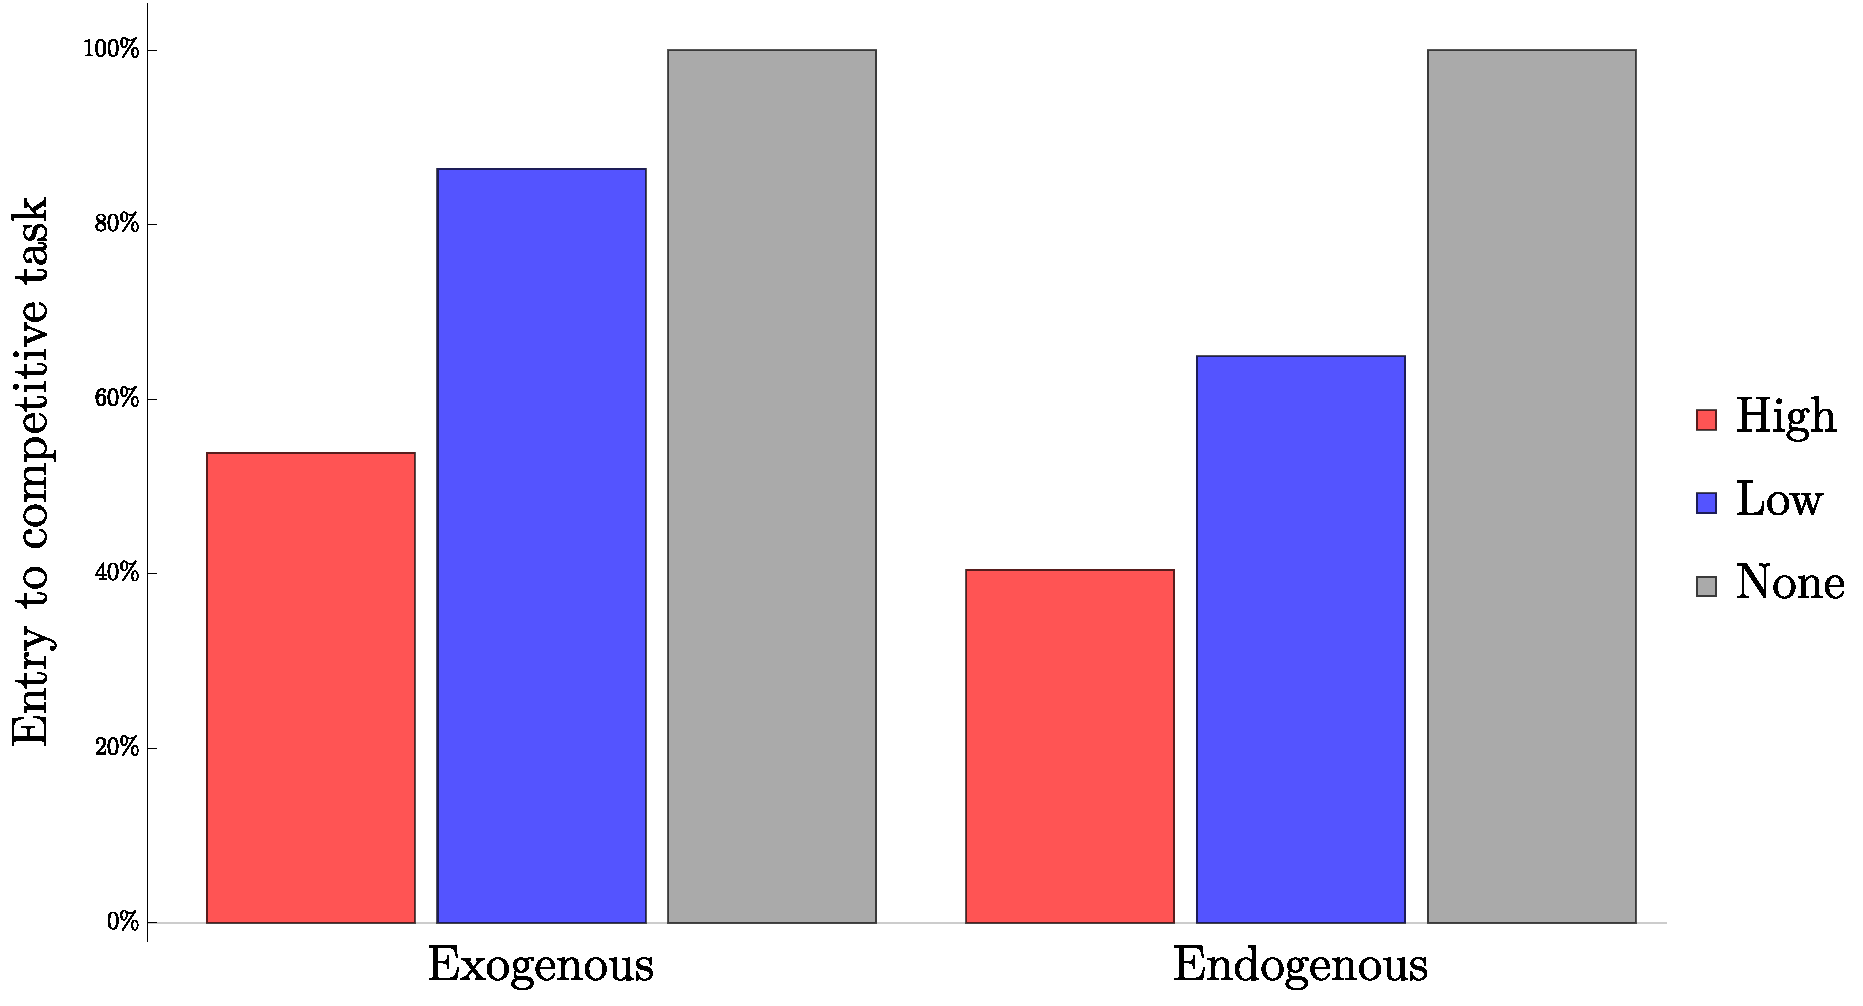
\includegraphics[width=0.8\textwidth]{./ih/col_TaskEntry.pdf}
    \end{center}
\end{frame}

\begin{frame}{Reports: No Outside Option}
    \begin{center}
        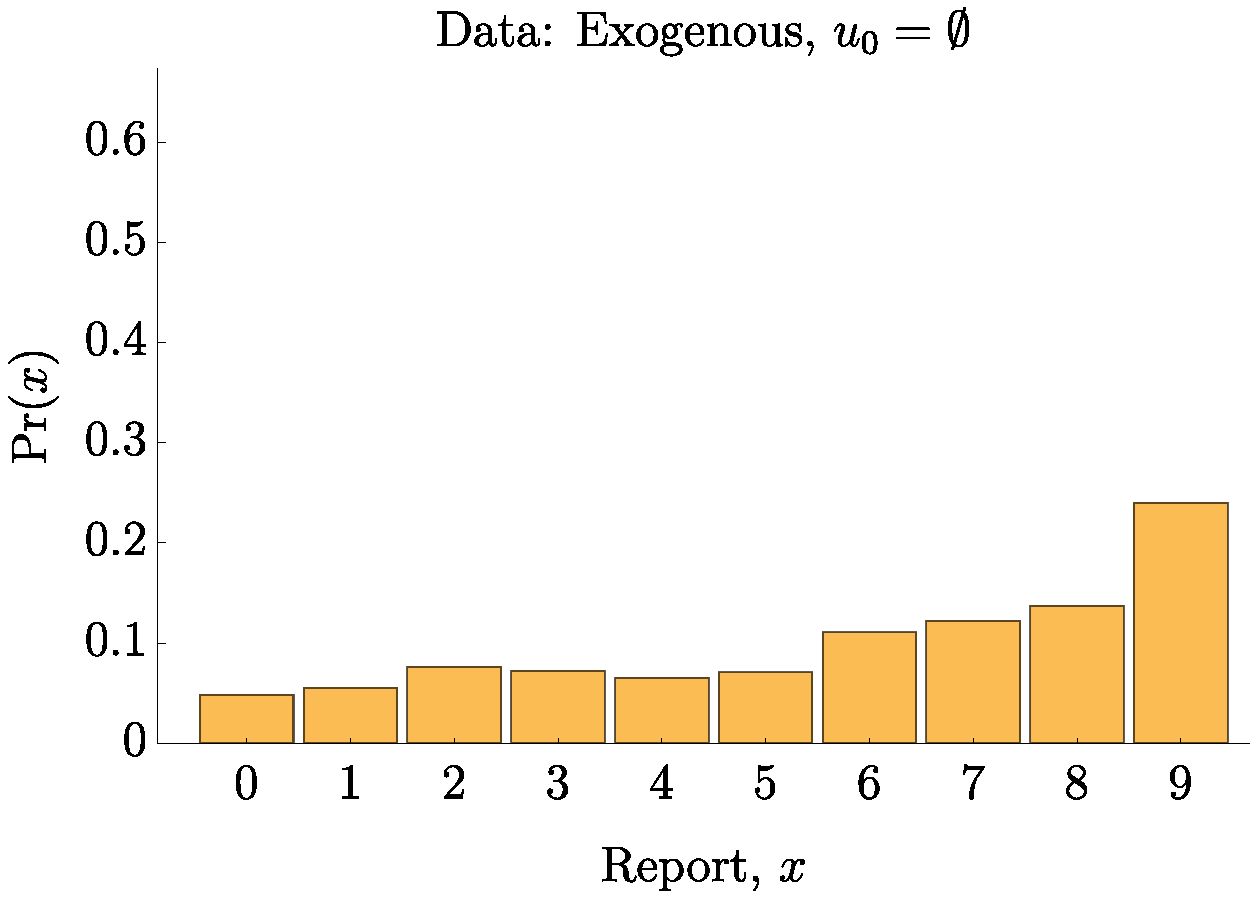
\includegraphics[width=0.5\textwidth]{./ih/emp_hist_ex_none.pdf}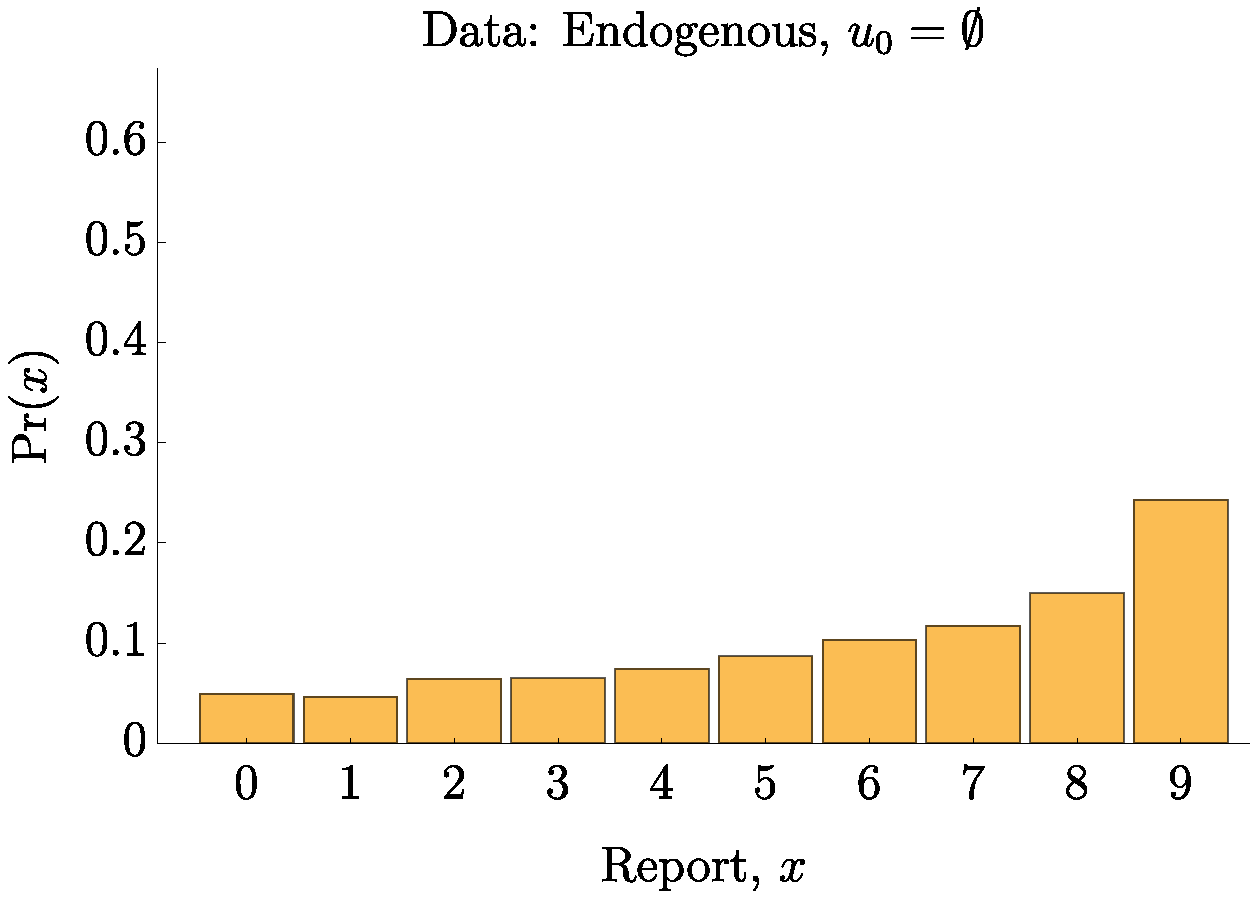
\includegraphics[width=0.5\textwidth]{./ih/emp_hist_en_none.pdf}
    \end{center}
\end{frame}

\begin{frame}{Reports: Exogenous prize}
    \begin{center}
        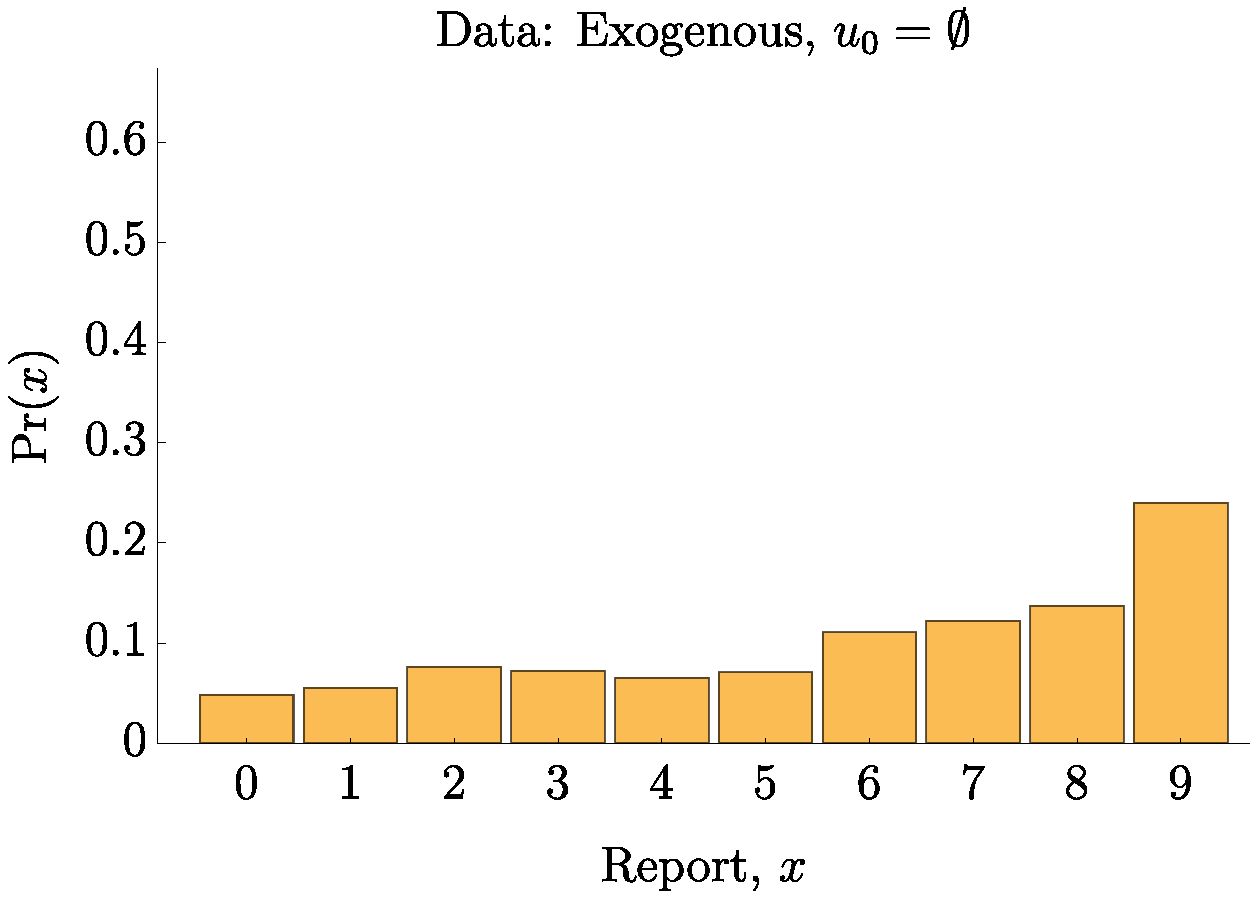
\includegraphics[width=0.32\textwidth]{./ih/emp_hist_ex_none.pdf}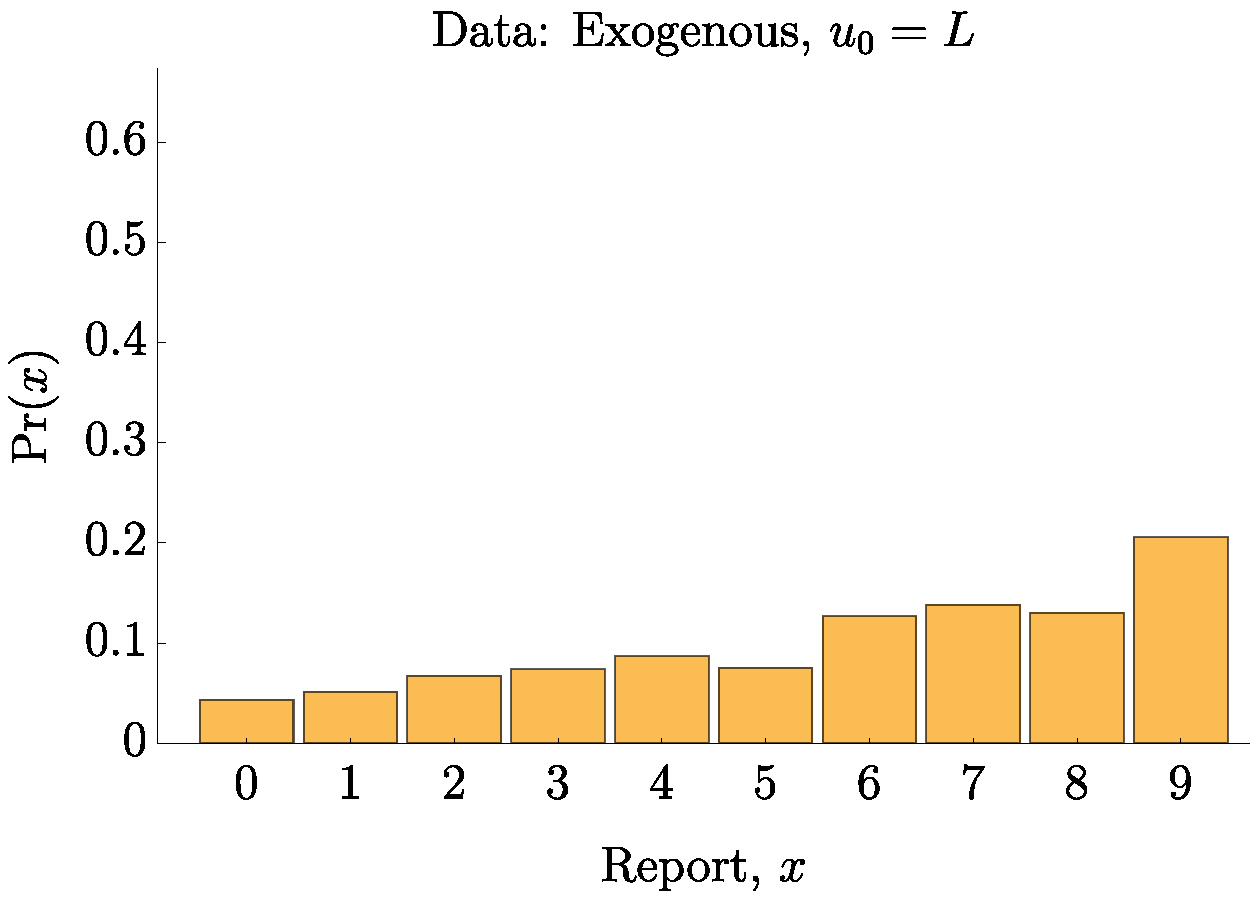
\includegraphics[width=0.32\textwidth]{./ih/emp_hist_ex_L.pdf}
        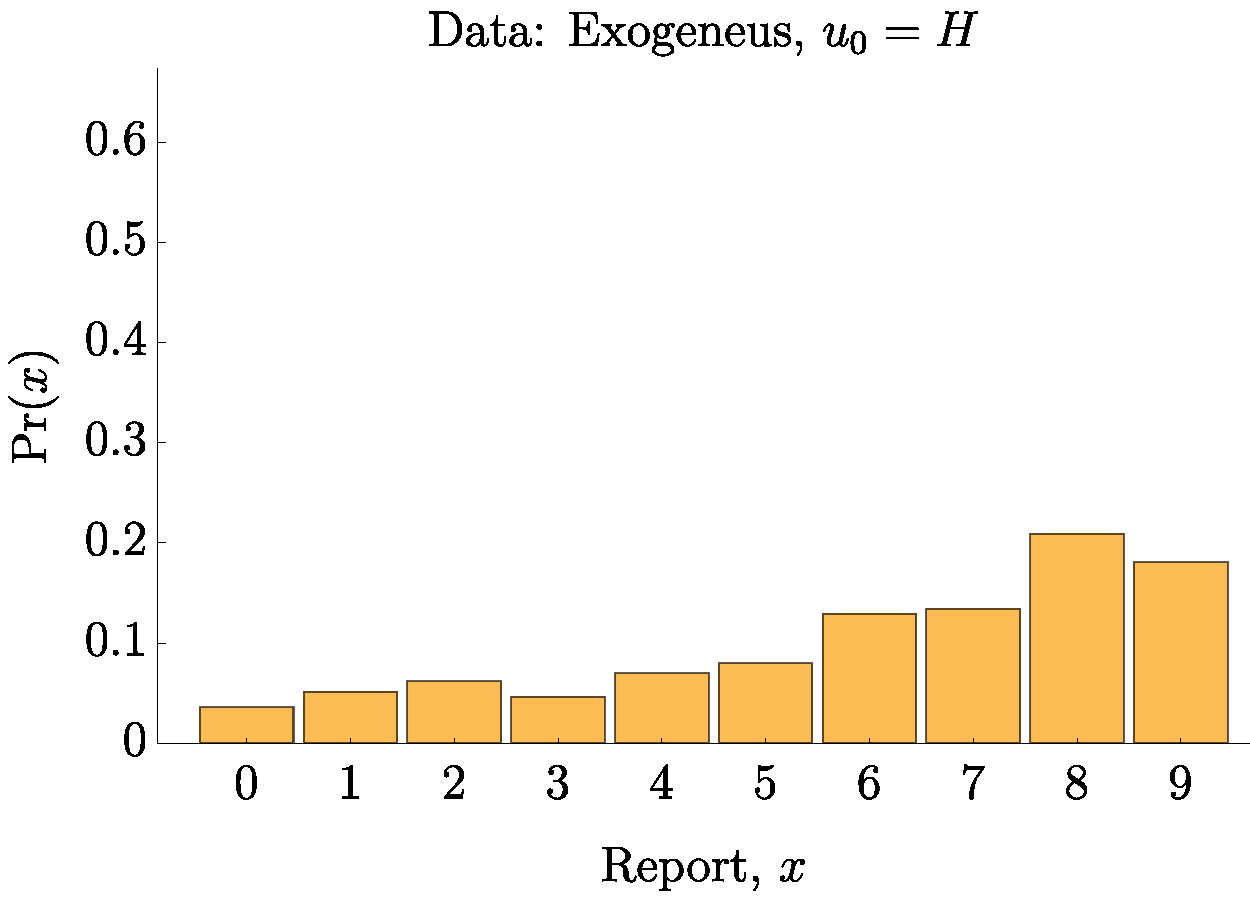
\includegraphics[width=0.32\textwidth]{./ih/emp_hist_ex_H.pdf}
    \end{center}
\end{frame}

\begin{frame}{Reports: Both}
    \begin{center}
        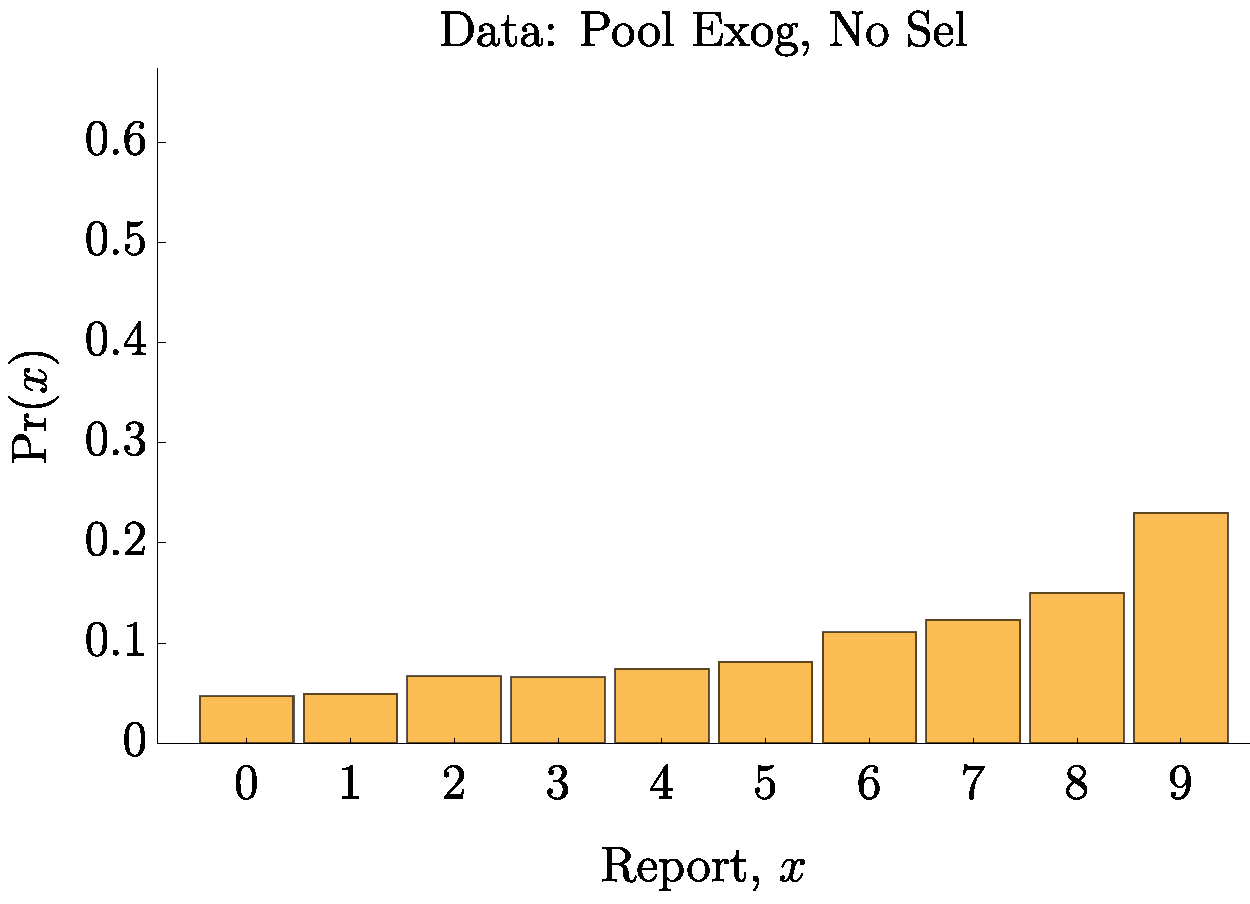
\includegraphics[width=0.32\textwidth]{./ih/emp_hist_pool.pdf}
        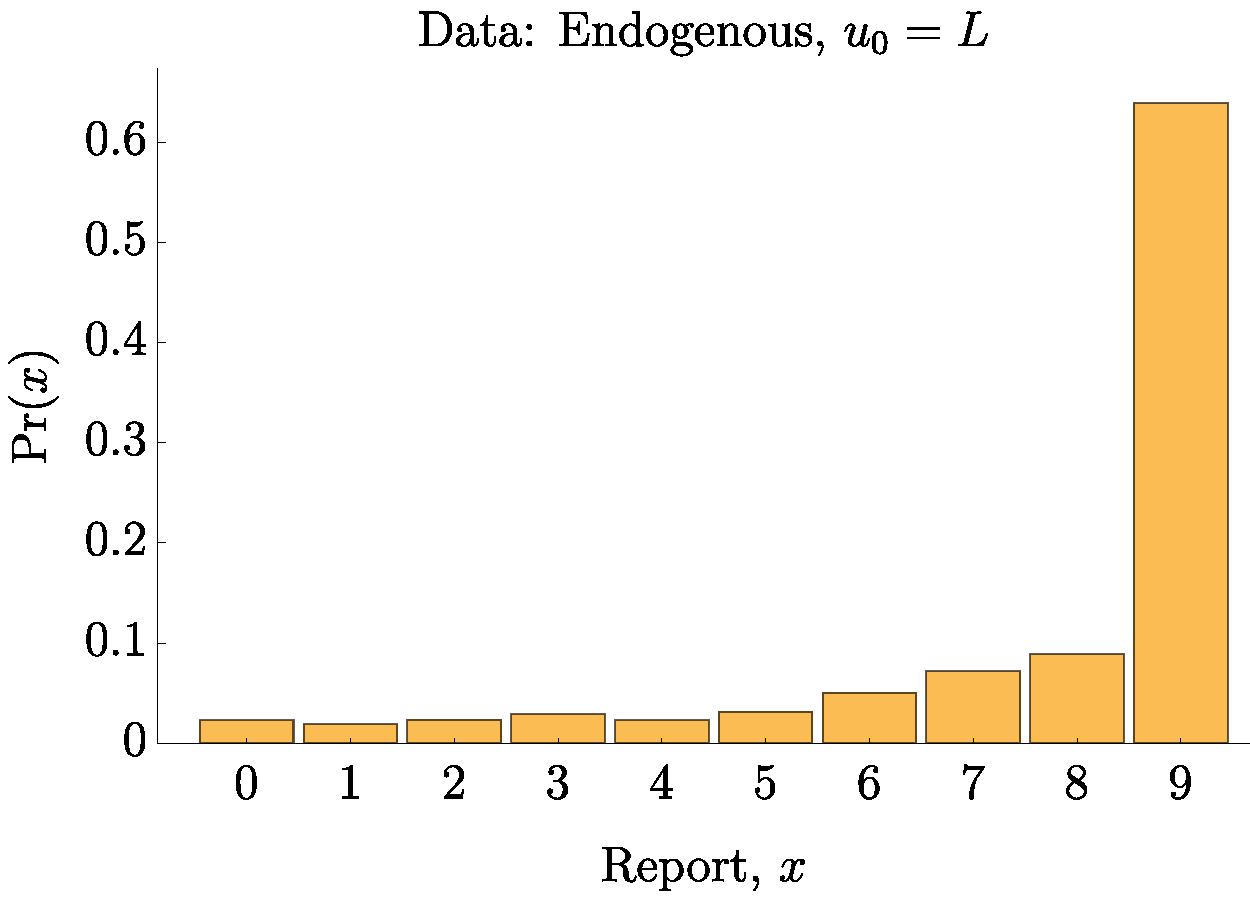
\includegraphics[width=0.32\textwidth]{./ih/emp_hist_en_L.pdf}
        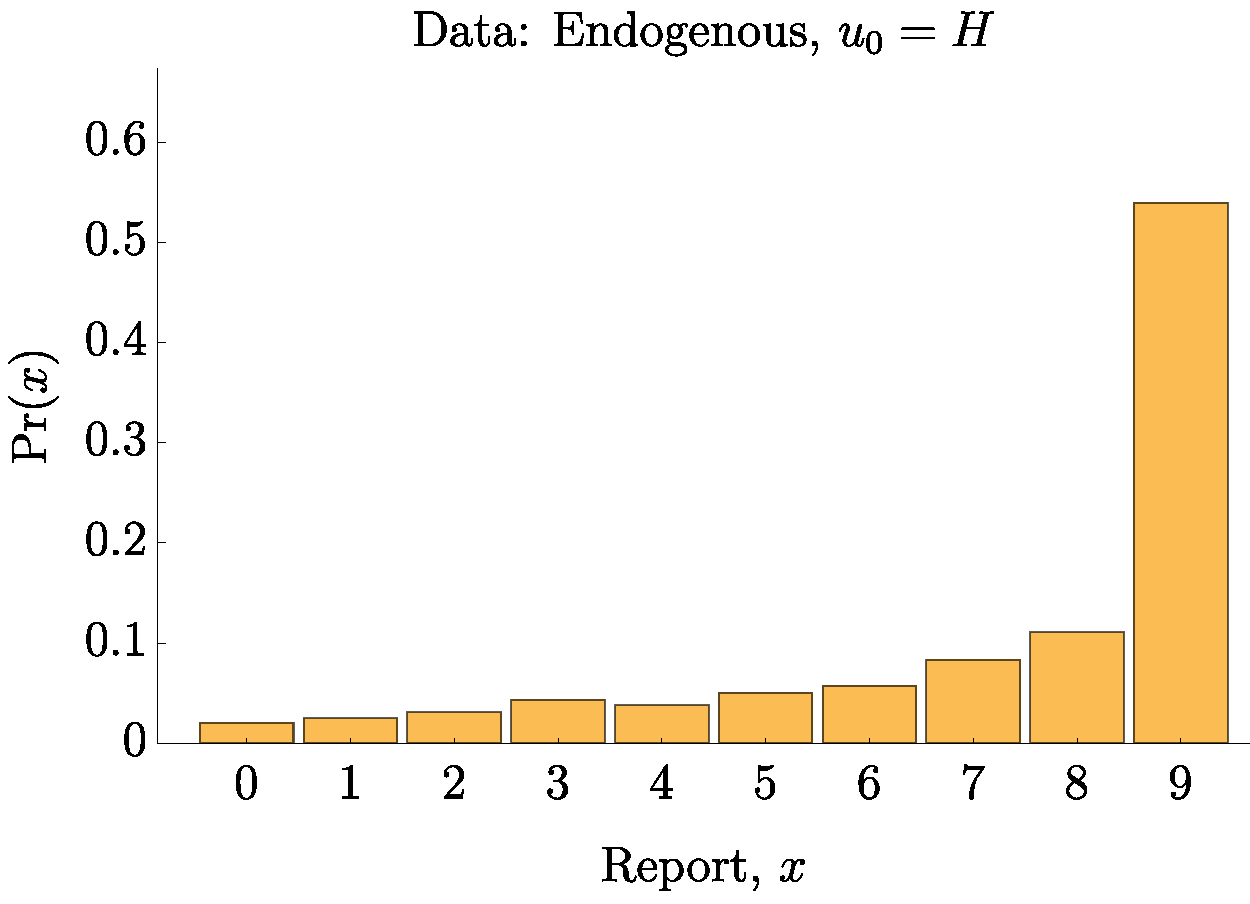
\includegraphics[width=0.32\textwidth]{./ih/emp_hist_en_H.pdf}
    \end{center}
\end{frame}

\begin{frame}{Results}
    \begin{center}
        \begin{tabular}{cccccccc}
        \toprule \textbf{Variable} & \multicolumn{3}{c}{\textbf{Exog-$\pi$}} &  & \multicolumn{3}{c}{\textbf{Endog-$\pi^{\star}$}}\\ 
        \cmidrule{2-4}\cmidrule{6-8} & \textbf{$\emptyset$} & \textbf{L} & \textbf{H} &  & \textbf{$\emptyset$} & \textbf{L} & \textbf{H}\\ 
        \midrule \textbf{Entry Rate} & 1 & 0.86 & 0.54 &  & 1 & 0.65 & 0.40\\ 
        \textbf{Fixed Report} & \textendash{} & 4.52 & 4.52 &  & \textendash{} & 4.72 & 4.58\\ 
        \textbf{Comp. Report} & 5.82 & 5.76 & 6.01 &  & 5.92 & 7.68 & 7.29\\ 
        \bottomrule
        \end{tabular}
    \end{center}
\end{frame}

\begin{frame}{Results}
    \begin{center}
        \begin{tabular}{cccccccc}
        \toprule \textbf{Variable} & \multicolumn{3}{c}{\textbf{Exog-$\pi$}} &  & \multicolumn{3}{c}{\textbf{Endog-$\pi^{\star}$}}\\ 
        \cmidrule{2-4}\cmidrule{6-8} & \textbf{$\emptyset$} & \textbf{L} & \textbf{H} &  & \textbf{$\emptyset$} & \textbf{L} & \textbf{H}\\ 
        \midrule \textbf{Entry Rate} & 1 & 0.86 & 0.54 &  & 1 & 0.65 & 0.40\\ 
        \textbf{Fixed Honesty} & \textendash{} & 1.00 & 1.00 &  & \textendash{} & 0.95 & 0.98\\ 
        \textbf{Comp. Honesty} & 0.71 & 0.72 & 0.66 &  & 0.68 & 0.29 & 0.38\\ 
        \bottomrule  &  &  &  &  &  &  & \\ 
        \end{tabular}
    \end{center}

Transform average reports to ``implied honesty'' via following:
\[
x\mapsto(9-x)/4.5
\]
\end{frame}

\begin{frame}{Results--Comparative Statics}
    \begin{center}
        \begin{tabular}{ccc}
        \toprule \textbf{Variable} & \multicolumn{2}{c}{\textbf{Joint Tests}}\\ 
        \cmidrule{2-3}  & $\boldsymbol{Ex}$ vs. $\boldsymbol{En}$ & \textbf{$\emptyset$} vs. $\boldsymbol{L}$ vs. $\boldsymbol{H}$\\ 
        \midrule \textbf{Entry Rate} & $\boldsymbol{Ex}{\color{red}\stackrel{\star\star\star}{\succ}}En$ & $\boldsymbol{L}{\color{red}\stackrel{\star\star\star}{\succ}}\boldsymbol{H}$\\ 
        \textbf{Fixed Honesty} & $\boldsymbol{Ex}\sim\boldsymbol{En}$ & $\boldsymbol{L}\sim\boldsymbol{H}$\\ 
        \textbf{Comp. Honesty} & $Ex{\color{red}\stackrel{\star\star\star}{\succ}}En$ & $\boldsymbol{\emptyset}{\color{red}\stackrel{\star\star\star}{\succ}}\boldsymbol{L}\sim\boldsymbol{H}$\\ 
        \bottomrule  &  & \\ 
        \end{tabular}
    \end{center}
\end{frame}

\begin{frame}{Aggregate Result}\begin{center}

\textbf{Result: }The interaction of selection with endogenous payoffs
substantially reduces honest revelation, with minimal effects from
each separate term.
\end{center}

\[
\hat{\lambda}=\underset{(0.062)}{0.706}-\underset{(0.076)}{0.007}\cdot\text{Sel}-\underset{(0.072)}{0.023}\cdot\text{En-}\ensuremath{\pi}-\underset{(0.090)}{0.349}\cdot\text{Sel\ensuremath{\times\text{En-\ensuremath{\pi}}.}}
\]
\end{frame}

\begin{frame}{Subject-level calculation}
    \begin{itemize}
        \item Above we looked at aggregate data, can instead look at the subject
        level
        \item For each subject with at least 5 rounds in the competitive task, we
        calculate their implied honesty:
            \begin{itemize}
                \item $\lambda_{i}=\frac{2}{9}\left(9-\frac{1}{\#Comp.}\sum x_{it}^{\text{Comp}}\right)$
                \item Then look at the smoothed distribution of $\lambda_{i}$
            \end{itemize}
    \end{itemize}
\end{frame}

\begin{frame}{Subject average honesty}
    \begin{center}
    	\includegraphics<1>[width=0.9\textwidth]{./ih/col_indivHonesty.pdf}
    \end{center}
\end{frame}

\begin{frame}{Group Dynamics}
    \begin{center}
    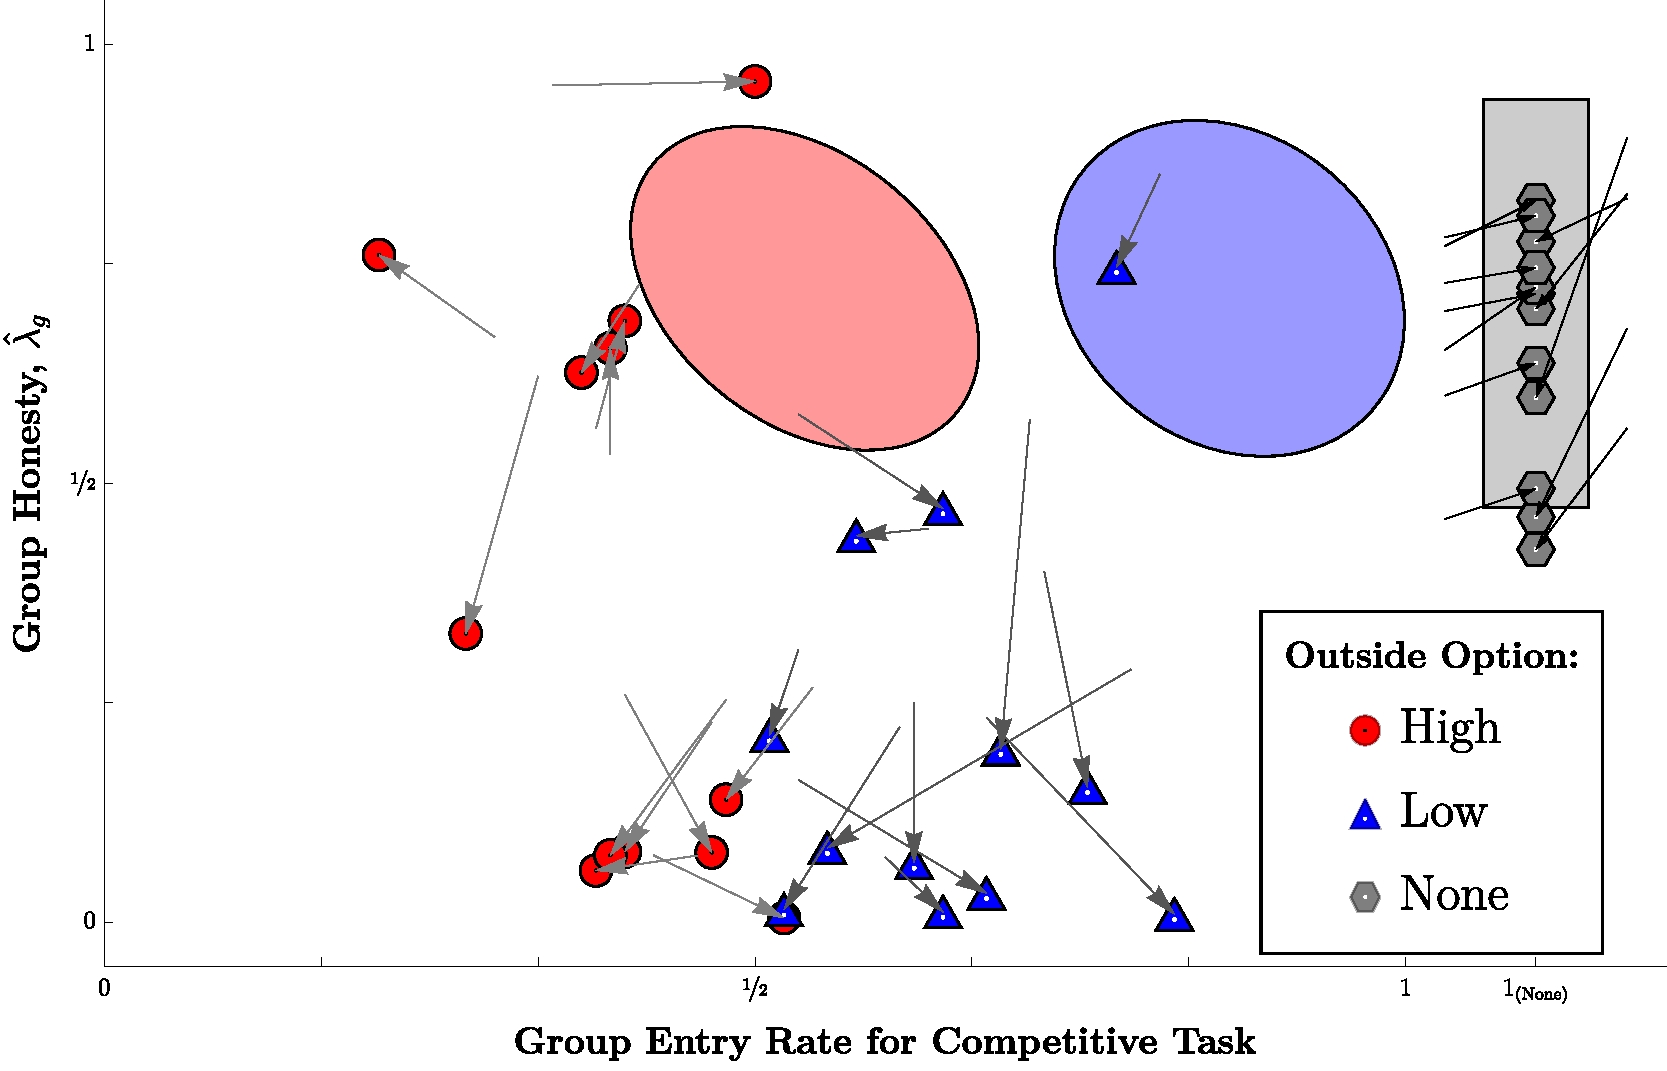
\includegraphics[width=0.8\textwidth]{./ih/col_Scatter_Group_WithArrowsEllipse.pdf}
    \end{center}
\end{frame}


\begin{frame}{Conclusions}
    \begin{itemize}
        \item Look at a repeated honesty task with task selection and competition
        \item Without \textbf{both} selection and prize endogeneity, our task leads
        to very similar results to the standard literature
        \item With \textbf{both} aggregate responses are much closer to the payoff-maximizing
        predictions
        \item Heterogeneity in the group results suggests a critical threshold below
        which our matching groups spiral down towards complete dishonesty
            \begin{itemize}
                \item Smaller communities more bi-modal
            \end{itemize}
        \item Reputational models do well at helping us understand the data across
        treatments
            % \begin{itemize}
            %     \item That said, they're computationally very complex
            % \end{itemize}
    \end{itemize}
\end{frame}

\end{document}
